\documentclass[homework]{IEEEtran}
\IEEEoverridecommandlockouts
% The preceding line is only needed to identify funding in the first footnote. If that is unneeded, please comment it out.
\usepackage{cite}
\usepackage{CJKutf8}
\usepackage{indentfirst}
\usepackage{amsmath,amssymb,amsfonts}
\usepackage{algorithmic}
\usepackage{graphicx}
\usepackage{textcomp}
\usepackage{xcolor}
\usepackage{hyperref}
\usepackage[justification=centering]{caption}
\setlength{\parindent}{2em}
\def\BibTeX{{\rm B\kern-.05em{\sc i\kern-.025em b}\kern-.08em
    T\kern-.1667em\lower.7ex\hbox{E}\kern-.125emX}}
\begin{document}

\title{Homework of Pattern classification II\\
{\footnotesize \textsuperscript{*}Name: Xue Yuan  | Student number: 202228015926034}
}

\author{}
\maketitle

\begin{abstract}
This document is about the first homework for Pattern classification by \LaTeX.
\end{abstract}

\section{calculation}
\begin{CJK}{UTF8}{gkai}
    \begin{enumerate}
		\item 一维特征空间中的窗函数为标准正态分布的概率密度函数$p(x)$的Parzen窗估计$p_n(x)$:  $$ p_n(x)=\frac{1}{n} \sum_{i=1}^n \frac{1}{\sqrt{2 \pi}} \exp \left(-\frac{(x-x_i)^{2}}{2}\right) $$
		\item 给定一维空间三个样本点$\{-4,0,6\}$,请写出概率密度函数$p(x)$的最近邻$(1-NN)$估计,并画出概率密度函数曲线图: \par
		(1)概率密度函数:  \par
        由:$$p_{1}(\mathbf{x})=\frac{k_{n}}{n V_{n}}=\frac{1}{2 n\left|x-x_{1}\right|}$$
        可得:$$p_{n}(x)=\frac{k_{n}}{n V_{n}}=\left\{\begin{aligned}
            &\frac{1}{6|x+4|},  & \text { if } x<-2&\\
            &\frac{1}{6|x|},    & \text { if }-2<x<3& \\
            &\frac{1}{6|x-6|},  & \text { if } x>3&
            \end{aligned}
            \right.$$
        (2)概率密度图像:
            \begin{figure}[htb]
                \centerline{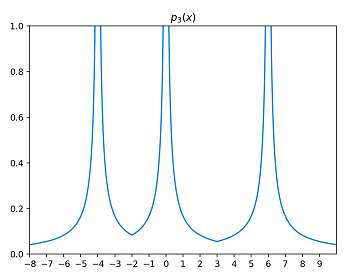
\includegraphics{Images/fig1.png}}
                \caption{Probability density function of 1-NN estimate}
                \label{fig}
            \end{figure}
        \item 现有7个二维向量:$x_1$=$(1,0)^T$,$x_2$=$(0,1)^T$,$x_3$=$(0,-1)^T$, \par
        $x_4$=$(0,0)^T$,$x_5$=$(0,2)^T$,$x_6$=$(0,-2)^T$,$x_7$=$(-2,0)^T$。
        这里上标$T$表示向量转置。假定前三个为$\omega_{1}$类, 后四个为$\omega_{2}$类。
        画出最近邻法决策面。\par
        由:$$g_{i}(\mathbf{x})=\arg \min _{\mathbf{x}_{j} \in \omega_{j}} d\left(\mathbf{x}, \mathbf{x}_{j}\right), \quad i=1,2, \ldots, c$$
        可作图:
        \begin{figure}[htb]
            \centerline{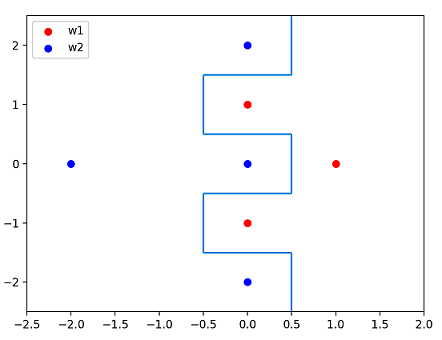
\includegraphics{Images/fig2.png}}
            \caption{Nearest neighbor decision surface}
            \label{fig} 
        \end{figure}
        \item 请给出K近邻分类器的优点和缺点。 \par
        (1) 其优点在于:算法理论简单,容易实现:准确性更高,对异常值和噪声有较高的容忍度    \par
        (2) 其缺点在于:k近邻算法每预测一个"点"的分类都会重新进行一次全局运算,对于样本容量大的数据集计算量比较大.而且K近邻算法容易导致维度灾难,在高维空间中计算距离的时候,就会变得非常远;此外,
        它还存在着难以区分样本数据存在部分重叠时的情况等等。 \par
        \item 解答过程如下:
        \begin{figure}[htb]
            \centerline{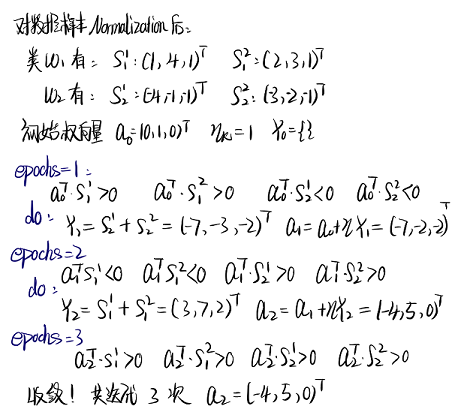
\includegraphics{Images/fig3.png}}
            \caption{Batch Perceptron flow chart}
            \label{fig} \par
        \end{figure}
    \end{enumerate}
\end{CJK}
\section{Programming}
\begin{CJK}{UTF8}{gkai}
    \begin{enumerate}[]
		\item 不同窗宽取值下所估计获得的概率密度函数曲线:\par
        \begin{figure}[htb]
            \centerline{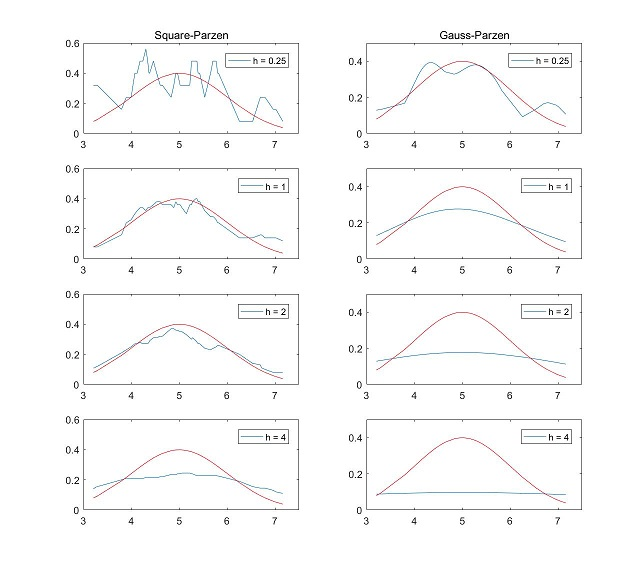
\includegraphics{Images/fig4.jpg}}
            \caption{Fitted images for two methods}
            \label{fig} \par
        \end{figure}
        图中蓝色线条是原始数据拟合得出,红色线条是$N(5,1)$的概率密度图像。可以看出窗大小$(h)$对拟合图像的好坏起到了十分明显的作用,并且不同的拟合方式对窗口大小的敏感成都也不同。本题所有代码均基于$Matlab$,源码放在附录中。
        \item 线性分类器的构造与训练 \par
        (1)当采用$Batch Perception$时,程序运行结果如下:\par
        \begin{figure}[htb]
            \centerline{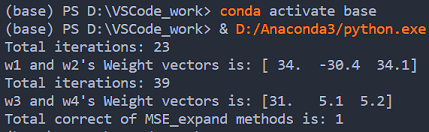
\includegraphics{Images/fig5.png}}
            \caption{Running result}
            \label{fig}
        \end{figure}  \par
        可以看出,他们的迭代次数分别是23和39。此外,图中还给出了两种分类情况下的权矢量值。 \par
        他们整体上的运行分类结果表示在附录中 \par
        (2)如图5所示,当采用$MSE_Expand$方法时,其测试集正确率达到了$100\%$!
        本题目代码基于$python3.9$,相关程序也在附录中展示。
    	\end{enumerate}\par
\end{CJK}

\section{Appendix}
\begin{CJK}{UTF8}{gkai}
    本次作业中,所采用的拟合计算代码均是基于Matlab和Python3.9,相关的源码已经被开源于Github上:
    \url{https://github.com/Alexiopro/First-year-of-UCAS/tree/main/UCAS/Source%20Code%20of%20Pattern%20Classification}
    供读者查用。 \par
    图fig6和fig7是Programming部分题(2)的第一小问中采用$Batch Perception$方法的运行展示。可以清晰的看出,采用$Batch Perception$方法处理数据的方式能够较好的划分数据的真实类别。
\end{CJK}
\begin{figure}[htb]
    \centerline{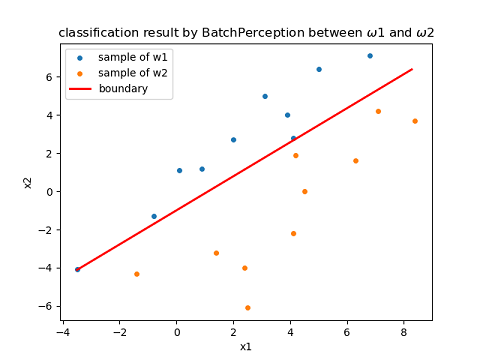
\includegraphics{Images/BP12.png}}
    \caption{W1 and W2 }
    \label{fig}
\end{figure}
\begin{figure}[htb]
    \centerline{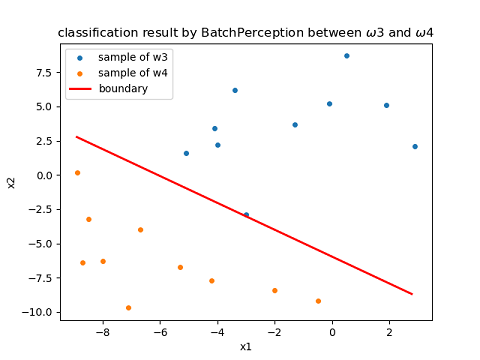
\includegraphics{Images/BP34.png}}
    \caption{W3 and W4}
    \label{fig}
\end{figure}\par

\end{document}
